\chapter{Introduction and History}\label{ch:intro}

%-----------------------------------
\section{Problem Statement}
The \ac{UAS} has evolved tremendously over the past decade.  Miniature autopilots have gotten smaller and cheaper with more sensitive and redundant sensor packages largely due to the cellular phone industry accelerating \ac{MEMS} technology.  The ability to manufacture these autonomous systems at fractions of the cost enables the advancement in multiple cooperative UAV applications including swarming capability.  This ability to mass-produce large quantities of \ac{UAS}'s poses an interesting challenge.  Even though the price has gone down and the performance has gone up, there still exists a significant amount of man-hours dedicated to sensor calibration and autopilot control law configuration and tuning for best achievable performance.  

The \ac{DoD} conducted an analysis of the role of autonomy, which outlined technology gaps and predicted advancements required to meet the growing performance demand of autonomy \cite{dodroadmap}.  The analysis amplifies the fact that autonomy is a difficult field and that it is arguably in its infancy.  The roadmap attempts to guide decision makers in ensuring capitalization of under-utilized technology and succinct awareness of technical challenges limiting the current state of the art.  Figure~\ref{fig:dod_roadmap} outlines these elements at increasing scope of control comprised of various technology portfolios.  
\begin{figure}[h!]
 \centering
  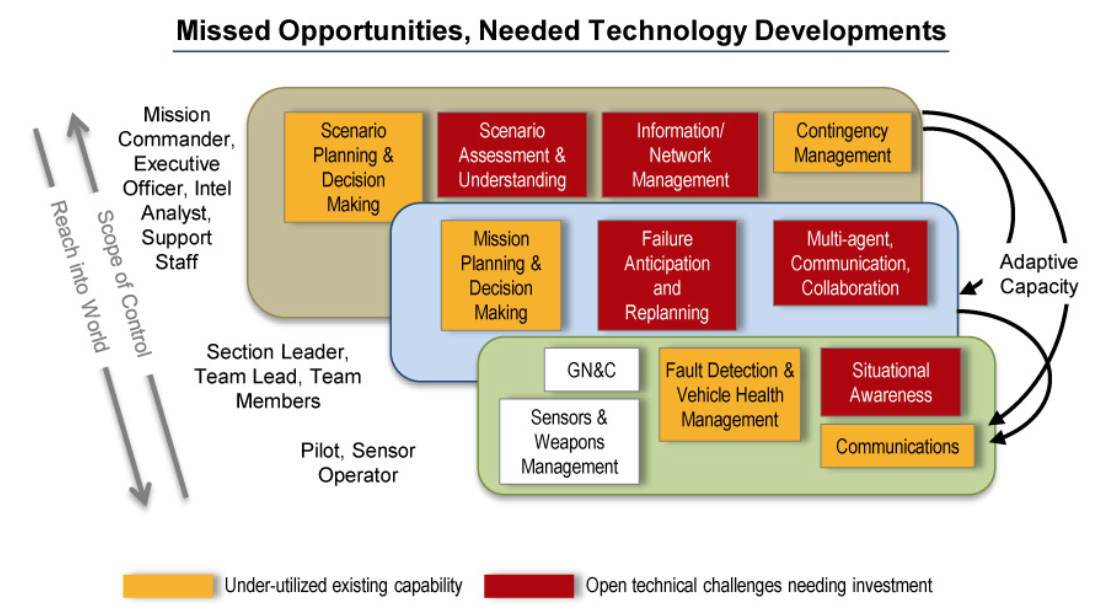
\includegraphics[width=1.0\textwidth]{DOD_roadmap.png}
  \caption{DoD Autonomy Roadmap \cite{dodroadmap}}
  \label{fig:dod_roadmap}
\end{figure}
The language referenced in the roadmap often recommends that machine learning and/or artificial intelligence is needed for elements such as "Fault Detection."  On the lowest level, the roadmap annotates the use of \ac{GNC} as neither needing improvement or current technology being underutilized.  An in-depth look at the current state of the art with respect to \ac{GNC} reveals that \ac{GNC} is still very costly and arguably antiquated.  Research of adaptive control as applied to \ac{GNC} offers new strategies offering improved performance and eventual reduced cost.

\ac{UAS} avionics have drastically improved over the past decade, but the fundamental control law algorithms have not changed.  The \ac{PID} architecture found it's origin in automatic ship steering applications in 1922 \cite{minorsky1922pid}.  Conventional control law architectures for \ac{UAS}'s predominately still use \ac{PID} controllers.  Conventional control law architectures for \ac{UAS}'s predominately still use \ac{PID} controllers.  Their architecture offers a well understood and predictable behavior and for this reason is well suited for the aviation application.  The detriment of \ac{PID} control is that its application is mostly constrained by its use on a linear plant and most aerospace applications are non-linear and time varying.   An aircraft's control authority that increases proportionally to dynamic pressure is one example of aerodynamic non-linear control behavior.  In this case, the \ac{PID} controller's robustness to changes in velocity and/or density altitude is not guaranteed and for most aircraft has to be delicately handled with lookup tables produced from hours of flight test.

Tuning the six to ten conventional \ac{PID} controllers for one airframe is not an insignificant task.  Swarming systems often will utilize the same airframe assembled by the same manufacturer, and all aircraft still require a tedious quality assurance check.  Physical aspects of the airframes such as \ac{CG}, control surface deflection/calibration/speed, airframe alignment, etc. all can drastically vary within the same delivered batch of airframes.  It should also be considered that most of these miniature \ac{UAS}'s experience hard landings, crashes, and/or damage in transportation, which all can affect aerodynamic handling qualities.  In summary, conventional control laws require a moderate to high level of expertise and require significant man-hours to tune properly for every airframe even if identical.  


%-----------------------------------
\section{Adaptive Control History}\label{history}
Adaptive control saw it's early debut in the NASA North American X-15 hypersonic rocket-powered X-plane experimental aircraft.  The X-15's performance envelope exceeded Mach 6.0 and 300,000 feet \cite{jenkins2000x15specs}.  Engineers realized early on that the linear controllers performed well only at one dynamic pressure, but nowhere near the entire flight envelope.  Scheduling the controller gains with respect to dynamic pressure (gain scheduling) was one method used to help ensure robustness;  the method is still widespread in commercial aviation due to its robustness but requires a lot of effort to 'explore' the entire flight envelope.  This was when the initial benefits of adaptive control were becoming realized.

The X-15 program started in 1959 and continued to 1968 flying nearly 200 successful flights.  It was considered one of NASA's most successful programs.  The benefit of adaptive control to the X-15 was that the adaptive controller was supposed to adjust the gain parameters online automatically.  If the controller was self-tuning, it could potentially offer increased performance while reducing complexity.  The Honeywell MH-96 adaptive controller was implemented in the X-15-3 as a fly-by-wire controller designed to adaptively adjust the damping in pitch and roll with respect to the desired model response.  The goal was to achieve consistent aircraft response regardless of dynamic pressure and other variables.  During test flights of the MH-96 adaptive control, increased performance was observed especially in the dynamic phases of reentry over that of the linear fixed gain damping system \cite{dydek2010adaptive}.  These early breakthroughs in adaptive control proved the benefits could be viable aerospace solutions.  However, on November 15, 1967, there was a fatal accident caused by the adaptive controller.  The adaptive controller created an out of control flight situation resulting in dynamic pressures exceeding the structural limits and subsequent breakup of the airframe at 65,000 feet.

The turbulent start of adaptive control as implemented on the X-15 program was largely due to the early naive understanding of robustness.  Contemporary robust adaptive control strives to encapsulate these deficiencies of robustness in studies and proofs using Lyapunov stability analysis.  In addition to the developments of rigorous stability tools, a number of unique techniques have also been implemented to further increase controller robustness although.  One such technique utilizes dead band limits on the model adaptation process to avoid system/measurement noise from causing the un-learning of the states \cite{lavretsky2013robust}.  The \Lone adaptive control algorithm utilizes a technique which seeks to decouple the adaptation rate from robustness by 'low pass filtering' the contribution of the fast estimator under the premise that estimating the entire frequency spectrum is overly ambitious and should be limited to the bandwidth of the actuator.  Many advances have been made in the adaptive control field over the past few decades and this research sets out to evaluate a small subset of these techniques in the unforgiving aerospace environment.





